\section{System Design}

\subsection{System Overview Diagram}

Figure \ref{fig:deployment} shows the deployment diagram for FANS. There will be three devices which communicate with
each other on a local network: the alarm system on a Raspberry Pi 4, a smoke detection and temperature logging system
on a second Raspberry Pi 4, and a notification system on a third Raspberry Pi 4. When the smoke detection system
detects smoke above the limiting threshold, it will signal the alarm system to sound the alarm. It will signal the
notification system to send out notifications to the affected persons. The smoke detection and temperature logging
system will also update the cloud database (hosted by Firebase) with the recorded smoke and temperature levels, and
enable a flag that indicates the emergency. The fourth device, the Pi Pico, will buzz when the cloud database indicates
that an emergency has been detected by the detection system. This will notify the user of the emergency.

The notification and alarm system are on separate devices to preserve their integrity in the case of an emergency. It
is possible that the smoke detection system will be closer to the source of the fire, and therefore be at risk of being
damaged/disabled. With the notification and alarm systems on separate devices connected through a local internet
connection, they will be able to perform their responsibilities with less risk of being damaged by flames.

The cloud database is a real-time database to facilitate the real-time nature of display information on the web GUI. In
addition, it will allow the haptic feedback device to buzz as soon as the smoke detection system signals an emergency
to the cloud database.

\begin{figure}[H]
    \centering
    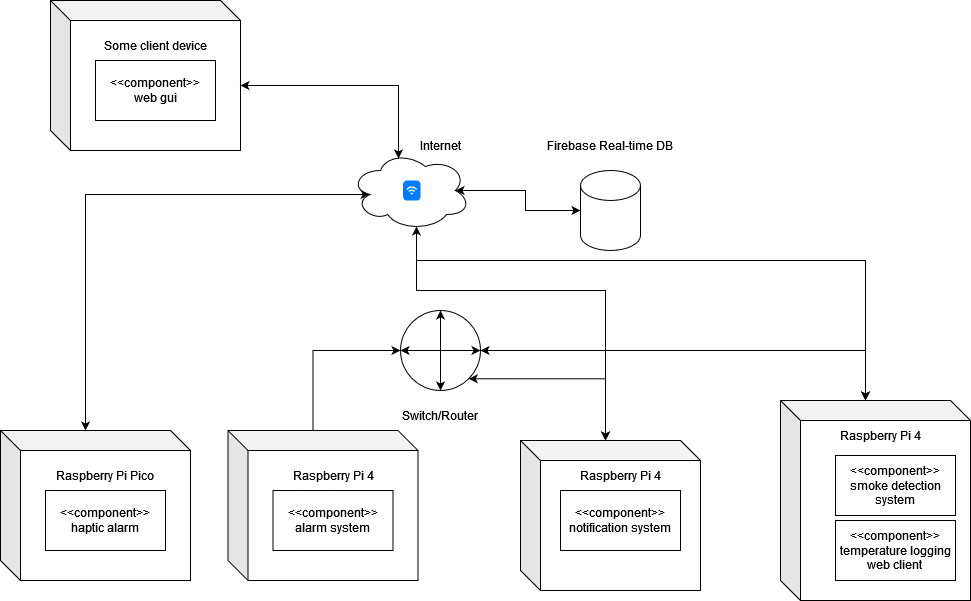
\includegraphics[width=\linewidth]{../assets/FANSDeployment.png}
    \caption{Deployment diagram of FANS.}
    \label{fig:deployment}
\end{figure}

The web GUI is displayed as being on the client device, because it will be accessible by any device with an internet
connection. It will be served on the cloud.

This configuration would allow us to scale our system horizontally very easily. Multiple different alarm systems and
smoke detectors could be connected over a local network to a notification system, allowing smoke detection in multiple
rooms and alarms sounding in multiple rooms. Additionally, several haptic alarm wearables could be clients to the
real-time database, allowing any number of users to be notified haptically in the event of an emergency.

Each subsystem has a single responsibility that allows for modularity in FANS. The alarm system simply waits to receive
a notification to sound its alarm, and then does so. The smoke detection and temperature sensing system periodically
writes sensor data to the real-time database, and also signals the database and the local notification system when it
detects a smoke or temperature measurement above the emergency threshold. The notification system is responsible for
receiving notice from the smoke detection system of an emergency, and then signalling the alarm system and sending
SMS/emails to all affected users in the database. The wearable haptic alarm system simply waits to be signalled by the
real-time database. Each subsystem has a clearly defined interface with specific messages passed between them, allowing
subsystems to operate without knowledge of each others’ implementations.

\subsubsection{Communication Protocols}

The smoke detection system will be communicating with an array of temperature and smoke sensors using the I2C protocol
over the GPIO pins of a Raspberry Pi 4.

Each node on the local network (the smoke detection system, alarm system and notification system) will communicate with
each other using UDP packets over the local network.

Nodes which communicate with the cloud hosted real-time Firebase database will use HTTP requests to interact with the
database. The smoke detection system will post JSON payloads to the database to write data. The web GUI will request
JSON over HTTP to update its visual components (dashboard with charts, etc.) with the data stored in the database. The
notification system will request contact information from the database over HTTP to send notifications to affected
users.

Finally, the notification system will communicate with affected users over email and SMS text notifications.

\subsection{Component Details}

The following section will describe the interfaces and responsibilities of each major node in the FANS system.

% TODO: Each of these subsubsections requires a sequence diagram
\subsubsection{Smoke Detection System} % TODO: I'm doing this one

The first component in the proposed system is the smoke detection and temperature sensing system. It will read sensor
data from a locally connected smoke sensor and temperature sensor using the I2C protocol over the Raspberry Pi 4's GPIO
pins. It will then update the real-time Firebase database with the collected sensor data over an internet connection.
If any temperature or smoke measurements are above the critical threshold for signalling an emergency, it will send a
message to the notification system and the alarm system over TCP to signify an emergency.

\begin{figure}[H]
    \centering
    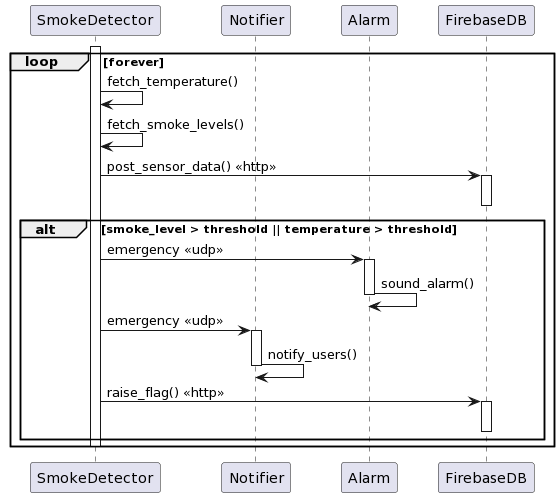
\includegraphics[width=5in]{../assets/SmokeDetectorSequence.png}
    \caption{Sequence diagram for the primary responsibilities of the smoke detector system.}
\end{figure}

\subsubsection{Notification System}

The notification system is responsible for notifying affected users of an emergency and triggering the alarm system. It
will also send SMS and email notifications to all users in the database to notify them of the detected emergency.

\subsubsection{Alarm System}

The alarm system is responsible for sounding an alarm in the building when an emergency has been detected. The alarm
system receives notification over TCP from the notification system when an emergency has been detected, at which point
it sounds an alarm and flashes lights. The lights will be an onboard SenseHat, and the alarm is still to be decided.
The alarm will continue to sound until the system receives a TCP message to stop.

\subsubsection{Haptic Alarm System} % TODO: I'm doing this one

The haptic alarm system is designed to be a wearable device that vibrates during an emergency. The device queries the
real-time database for a flag indicating an alarm. Once the flag is raised, the device vibrates until the emergency has
ended (the flag is “lowered”).

\subsubsection{Firebase Real-time Database} % TODO: I'm doing this one

The real-time database is responsible for storing smoke and temperature level data in real-time, as well as a database
flag indicating emergency. User contact information will also be stored in this database. Finally, it will also contain
user-configured settings (such as smoke level threshold for triggering an emergency). It will be cloud hosted by
Firebase.

\subsubsection{Web GUI}

The web GUI is responsible for displaying the sensor information from the real-time database. It will also allow users
to configure settings for FANS (emergency thresholds, etc.) and add more user contact information in the case of an
emergency. It will also allow users to disable the alarm when an emergency has been resolved.

\subsection{Use Cases}

\subsubsection{Trigger Emergency}

\textbf{Flow of events}
\begin{enumerate}
    \item The smoke detection system sends a TCP message to the notification system to warn of an emergency.
    \item The smoke detection system raises a flag in the real-time database to indicate the emergency.
    \item The notification system forwards this message to the alarm system.
    \item The notification system begins sending SMS and email notifications to the users who are listed in the database.
    \item The alarm system receives the TCP message from the notification system.
    \item The alarm system sounds the alarm and flashes LEDs.
    \item The haptic alarm system reads the flag from the real-time database.
    \item The haptic alarm system begins buzzing.
\end{enumerate}
